\documentclass[9pt,a4paper,twocolumn,twoside]{tau-class/tau}
\usepackage[ngerman]{babel}
\usepackage[T1]{fontenc}
\usepackage{graphicx}
\usepackage{booktabs}
\usepackage{siunitx}
\usepackage{tabularx}
\usepackage{array}
\usepackage{enumitem}
\usepackage{float}
\usepackage{pdfpages}
\newcommand{\pairfigwidth}{0.47\textwidth}

\begin{document}

\hypersetup{pageanchor=false}

%----------------------------------------------------------
% Titelseite im Stil von main.tex, aber ohne doppelte Nennung
%----------------------------------------------------------
\begin{titlepage}
    \centering
    \vspace*{0.5cm}

    
\includegraphics[width=0.45\textwidth]{../Summary_Felix_N/figures/JLU_Giessen-Logo.png}\\[1.8cm]

    {\Large Gruppennummer: 308}\\[0.3cm]
    \rule{\linewidth}{0.2mm}\\[0.2cm]
    {\huge\bfseries Neuronales Netz f\"ur den kalifornischen Hauspreis-Datensatz}\\
    \rule{\linewidth}{0.2mm}\\[1.5cm]

    \begin{minipage}{0.52\textwidth}
        \begin{flushleft}
            \textbf{\large Portfolio von:}\\[0.3em]
            Florian Adamczyk\\
            Matrikelnummer: 8105234\\[1.0em]

            \textbf{Rolle im Projekt:}\\
            Vorarbeit, Infrastruktur, EDA, Baseline, Kern-Notebook NN
        \end{flushleft}
    \end{minipage}
    \begin{minipage}{0.44\textwidth}
        \begin{flushleft}
            \textbf{\large Gruppenmitglieder:}\\[0.3em]
            Bj\"orn Becker\\
            Felix Hollfoth\\
            Felix Neumann (Sprecher)\\
            Kolja Scriba\\[1.0em]

            \textbf{Projektfokus:}\\
            California Housing, klassische Verfahren und neuronale Netze
        \end{flushleft}
    \end{minipage}\\[1.7cm]

    \begin{minipage}{0.88\textwidth}
        \begin{center}
            Modul: K"unstliche Intelligenz I\\
            Dozenten: Prof. Dr. Christian Heiliger, Dr. Jan-Matthis Waack\\
            Semester: Wintersemester 2025/26\\
            Abgabetermin: 15.04.2026
        \end{center}
    \end{minipage}

    \vfill
\end{titlepage}

\clearpage
\hypersetup{pageanchor=true}
\pagenumbering{arabic}
\setcounter{page}{1}

\doctype{Zusammenfassung des Logbuchs}
\title{Neuronales Netz f\"ur den kalifornischen Hauspreis-Datensatz}
\author[a]{Florian Adamczyk}
\affil[a]{Justus-Liebig-Universit\"at Gie\ss{}en, Matrikelnummer 8105234}
\dates{Gruppe 308 -- KI~I Projekt WS~2025/26}
\footinfo{KI~I Portfolio}
\theday{\today}
\organization{JLU Gie\ss{}en}
\leadauthor{F. Adamczyk}

\begin{abstract}
Diese Zusammenfassung dokumentiert meinen konkreten Beitrag zum KI~I-Projekt zur Vorhersage von Hauspreisen im California-Housing-Datensatz. Der Schwerpunkt liegt auf der Vorarbeit, ohne die die anschlie\ss{}ende Gruppenarbeit nicht reproduzierbar gewesen w\"are: Repository-Initialisierung, Umgebungsmanagement, gemeinsame Python-Hilfsfunktionen, einheitliche Metriken, standardisierte Plots und der Einstieg in die Modellierung.

Der Arbeitsumfang in der ersten Version war inzwischen veraltet, weil das Logbuch sp\"ater noch deutlich erweitert wurde. Diese Fassung aktualisiert den Umfang und zeigt deshalb nicht nur das sp\"ate neuronale Netz, sondern auch die methodischen Grundsteine: EDA, Baseline, Regularisierung, Entscheidungsbaum, kNN, Ensemble-Modelle und die Hyperparameterarbeit rund um das Neuronale Netz.

Mein bestes neuronales Netz erreicht auf dem Testset einen $R^2$-Wert von 0{,}7795 und liegt damit klar \"uber der linearen Regression mit 0{,}6326. Entscheidend war dabei nicht nur das Modell selbst, sondern die saubere technische Grundlage, auf der die gesamte Gruppe arbeiten konnte.
\end{abstract}

\keywords{California Housing, Neuronales Netz, TensorFlow, Regression, Git, Reproduzierbarkeit}

\maketitle
\thispagestyle{firststyle}

%----------------------------------------------------------
\section{Fragestellung und eigener Beitrag}
%----------------------------------------------------------
Ziel des Projekts war es, den California-Housing-Datensatz so aufzubereiten und zu modellieren, dass die Vorhersage von \texttt{MedHouseVal} nicht nur mit klassischen Verfahren, sondern auch mit einem neuronalen Netz sinnvoll eingeordnet werden kann \cite{aufgabe,sklearnHousing}. Meine Rolle war dabei bewusst fr\"uh und technisch grundlegend: Ich habe das Repository initialisiert, die gemeinsame Umgebung vorbereitet, die Projektstruktur dokumentiert und die Basiskomponenten gebaut, auf denen die sp\"atere Gruppenarbeit aufsetzt.

Im Gegensatz zu reiner Modelloptimierung war mein Beitrag vor allem ein Reproduzierbarkeitsbeitrag. Ohne einheitlichen Daten-Split, konsistente Metriken, gemeinsame Plots und eine saubere Git-/Notebook-Disziplin w\"aren die Ergebnisse der verschiedenen Teammitglieder kaum direkt vergleichbar gewesen. Genau deshalb ist diese Vorarbeit fachlich relevant und nicht nur organisatorisch.

\begin{table}[H]
\centering
\caption{Meine Hauptbeitr\"age im Projektverlauf}
\label{tab:my_contribution}
\begin{tabularx}{\columnwidth}{>{\raggedright\arraybackslash}p{2.9cm}X}
\toprule
\textbf{Bereich} & \textbf{Inhalt} \\
\midrule
Repository/Setup & Git-Initialisierung, erste Struktur, nbstripout, VS-Code-Unterst\"utzung \\
Dokumentation & README, Ressourcen, Masterplan, Aufgaben\"ubersicht, Meeting-Vorlagen \\
Python-Basis & requirements.txt, kompatible Umgebung, gemeinsames \texttt{utils/} \\
Daten/Plots & Laden, Cleaning, Split, Metriken, Standardplots, Export nach results/ \\
Modelle & EDA, lineare Baseline, LASSO/Ridge, Decision Tree, kNN, NN \\
\bottomrule
\end{tabularx}
\end{table}

\section{Warum die Vorarbeit zentral war}
Die eigentliche Leistung meines Beitrags liegt darin, dass alle weiteren Notebooks auf derselben technischen Basis arbeiten konnten. Das betrifft drei Dinge besonders stark: denselben bereinigten Datensatz, dieselbe Trennung in Train und Test und dieselben Metriken. Dadurch sind Unterschiede zwischen Modellen nicht zuf\"allig durch verschiedene Splits oder unterschiedliche Auswertelogik verf\"alscht.

Zus\"atzlich war die Arbeit an README, Anforderungen und Team-Support wichtig, weil es f\"ur viele im Team das erste Projekt in dieser Umgebung war. Ich habe deshalb nicht nur Code geschrieben, sondern auch die Einstiegsh\"urde f\"ur die anderen reduziert: klare Struktur, laufende Umgebung, reproduzierbare Notebook-Workflows und Hilfe bei Git und VS Code.

\subsection*{Verwendete Hilfsmodule in \texttt{utils/}}
Die von mir geschriebenen Kernmodule waren \texttt{utils/data.py}, \texttt{utils/evaluation.py} und \texttt{utils/plotting.py}. Zusammen bilden sie die Infrastruktur, die alle weiteren Notebooks genutzt haben.

\small
\textbf{\texttt{data.py}}\par
\begin{itemize}[leftmargin=*,itemsep=0.12em,topsep=0.2em]
    \item \texttt{load\_raw\_data}: California-Housing-Datensatz als DataFrame laden.
    \item \texttt{clean\_data}: Cut-offs entfernen und Ausrei\ss{}er \'uber das 98\%-Quantil filtern.
    \item \texttt{load\_and\_clean\_data}: Laden und Bereinigen in einem Schritt.
    \item \texttt{get\_train\_test\_split}: Einheitlichen 80/20-Split erzeugen, optional skalieren.
\end{itemize}

\textbf{\texttt{evaluation.py}}\par
\begin{itemize}[leftmargin=*,itemsep=0.12em,topsep=0.2em]
    \item \texttt{evaluate\_model}: R\textsuperscript{2}, MAE und RMSE f\"ur Train und Test berechnen.
    \item \texttt{evaluate\_predictions}: Dasselbe direkt aus Vorhersagen, z.\,B. f\"ur Keras-Modelle.
    \item \texttt{evaluate\_test\_predictions}: Kompakte Testauswertung f\"ur Modelle mit nur Test-Output.
    \item \texttt{add\_result}: Ergebnis in die gemeinsame Vergleichsliste schreiben.
    \item \texttt{compare\_models}: Vergleichstabelle aller Modelle erstellen und sortieren.
    \item \texttt{reset\_results}: Ergebnisliste zur\"ucksetzen.
\end{itemize}

\textbf{\texttt{plotting.py}}\par
\begin{itemize}[leftmargin=*,itemsep=0.12em,topsep=0.2em]
    \item \texttt{save\_fig}: Einheitlicher Export als PNG und PDF nach \texttt{results/}.
    \item \texttt{plot\_predicted\_vs\_actual}: Soll-Ist-Streudiagramm mit Ideallinie.
    \item \texttt{plot\_residuals}: Residuen gegen Vorhersage.
    \item \texttt{plot\_feature\_importances}: Wichtige Features geordnet darstellen.
    \item \texttt{plot\_correlation\_heatmap}: Korrelationsmatrix als Heatmap.
    \item \texttt{plot\_histograms}: Histogramme aller Merkmale in einem Raster.
    \item \texttt{plot\_features\_vs\_target}: Scatterplots aller Features gegen \texttt{MedHouseVal}.
\end{itemize}
\normalsize

Diese Vorarbeit war f\"ur die Gruppe entscheidend, weil sie nicht nur Zeit gespart hat, sondern die gemeinsame Aussagekraft aller Experimente erst hergestellt hat. Modelle sind nur dann wirklich vergleichbar, wenn Datenaufbereitung, Split und Bewertung identisch sind.

\subsection*{Weitere Beitr\"age im Projektverlauf}
Neben der technischen Basis habe ich im Projektverlauf weitere Aufgaben \"ubernommen. Dazu geh\"orten die laufende Betreuung des Repositories, die Unterst\"utzung bei Git-Konflikten im Team, die Ausarbeitung von Vorlagen f\"ur Gruppentreffen, die Pflege der Abh\"angigkeiten in \texttt{requirements.txt} und sp\"ater die Bereitstellung eines gemeinsamen Tau-Templates f\"ur die Portfolio-Summarys.

Ein weiterer wichtiger Schritt war am Ende die bewusste Entscheidung, \texttt{nbstripout} tempor\"ar zu deaktivieren und die Notebooks mit gespeicherten Outputs zu committen, damit die Korrektur direkt alle Ergebnisse, Kurven und Metriken sehen kann \cite{nbstripout}. Genau dieser Wechsel zwischen sauberer Entwicklungshistorie und transparenter Abgabe war Teil meiner Koordinationsarbeit.

Die Logbuch-Eintr\"age zeigen au\ss{}erdem, dass diese Vorarbeit aus konkreten technischen Arbeitspaketen bestand: Am 11.02. habe ich nach dem ersten Gruppentreffen den Notebook-Git-Workflow recherchiert, \texttt{nbstripout} praktisch getestet und die zentrale Ressourcen-Dokumentation aufgebaut. Am 17.02. folgte die technische Konsolidierung mit \texttt{.gitattributes}, Aufr\"aumen fr\"uher Repo-Artefakte und Stabilisierung der gemeinsamen Struktur. Genau diese fr\"uhe Standardisierung hat in der Folge Setup-Zeit und Merge-Probleme im Team reduziert.

%----------------------------------------------------------
\section{Datenbasis und explorative Analyse}
%----------------------------------------------------------
Zu Beginn habe ich die Rohdaten untersucht, um die Struktur des Datensatzes zu verstehen und die sp\"atere Bereinigung nachvollziehbar zu machen. Besonders wichtig waren die bekannten Cut-offs bei \texttt{MedHouseVal} und \texttt{HouseAge} sowie die starken Ausrei\ss{}er in \texttt{AveRooms}, \texttt{AveBedrms}, \texttt{Population} und \texttt{AveOccup}. Genau diese Schritte wurden sp\"ater in \texttt{utils/data.py} zentralisiert.

\begin{figure}[H]
    \centering
    \includegraphics[width=\pairfigwidth]{../../results/eda_histograms_raw.png}
    \hfill
    
\includegraphics[width=\pairfigwidth]{../../results/eda_histograms_clean.png}
    \caption{Vorher-Nachher-Vergleich der Verteilungen aller Kernmerkmale. Links (raw) erkennt man die Probleme des Rohdatensatzes: harte Deckelungen und starke Rechtsschiefe, insbesondere bei \texttt{AveRooms}, \texttt{AveBedrms}, \texttt{Population} und \texttt{AveOccup}. Rechts (clean) ist nach den von mir implementierten Bereinigungsschritten (Cut-off-Behandlung und Quantilfilter) eine deutlich stabilere Verteilungsstruktur sichtbar. Diese Gegen\"uberstellung macht den Effekt meiner Vorarbeit direkt sichtbar: Die nachfolgenden Modelle werden weniger von Extremwerten dominiert und auf konsistenteren Eingaben trainiert.}
    \label{fig:eda-raw-vs-clean-hist}
\end{figure}

\begin{figure}[H]
    \centering
    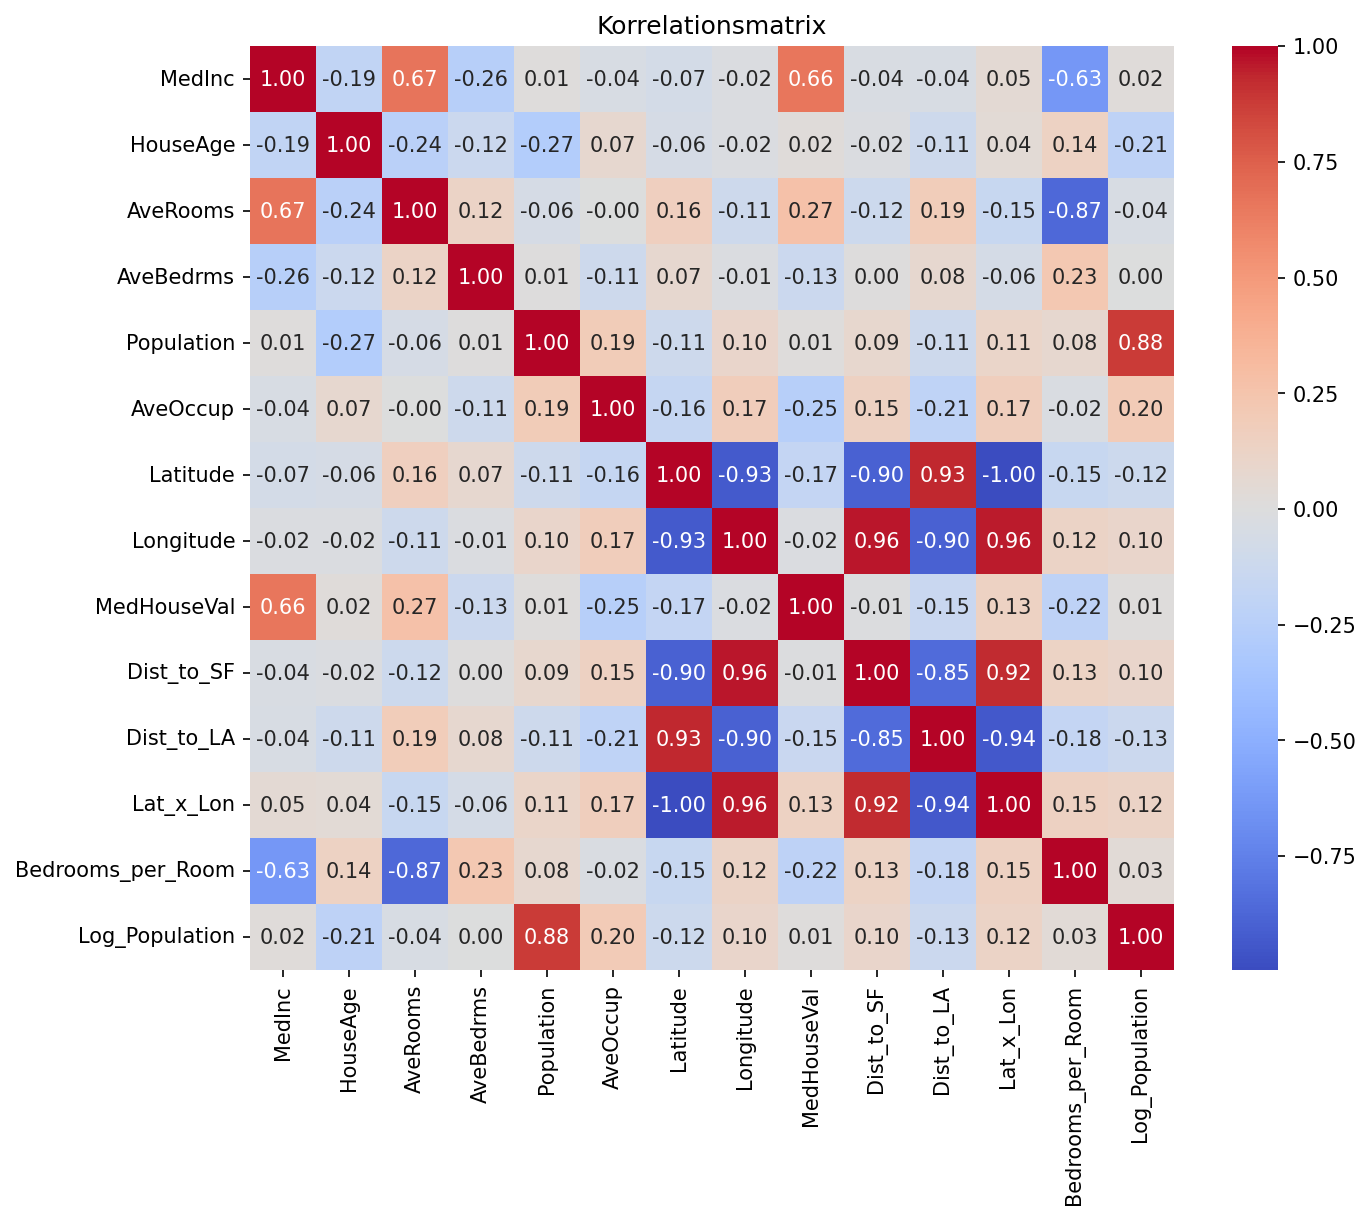
\includegraphics[width=\columnwidth]{../../results/eda_correlation_heatmap.pdf}
    \caption{Korrelationsmatrix der bereinigten Merkmale. Besonders klar ist der starke Zusammenhang zwischen \texttt{MedInc} und \texttt{MedHouseVal}; zugleich zeigen die weiteren Korrelationen, dass das Problem nicht rein eindimensional ist.}
    \label{fig:eda-corr-scatter}
\end{figure}

Die EDA war kein Selbstzweck. Sie hat direkt die Modellwahl vorbereitet: lineare Verfahren als Baseline, Regularisierung wegen Korrelationen, nichtlineare Verfahren wegen der sichtbaren Struktur und sp\"ater auch geographische und abgeleitete Merkmale. Die Plots zeigen au\ss{}erdem, warum das Problem nicht nur durch ein einzelnes lineares Signal erkl\"art werden kann.

%----------------------------------------------------------
\section{Von der Baseline zu klassischen Modellen}
%----------------------------------------------------------
Die lineare Regression war die erste belastbare Referenz. Sie hat als Minimum dienen sollen, gegen das alle weiteren Modelle gemessen werden. Der Residuenplot zeigt allerdings systematische Muster: Das Modell untersch\"atzt in bestimmten Preisbereichen und bildet komplexe Strukturen nur teilweise ab.

\begin{figure}[H]
    \centering
    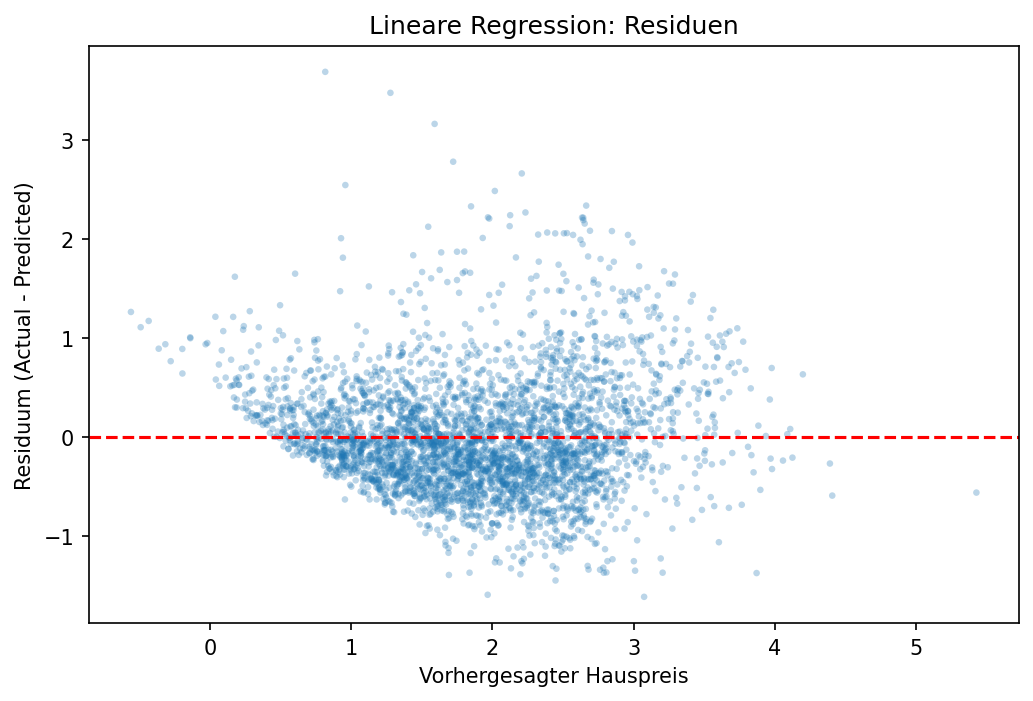
\includegraphics[width=\columnwidth]{../../results/baseline_residuals.pdf}
    \caption{Baseline mit linearer Regression: Residuenplot auf dem Testset. Die erkennbaren systematischen Fehler zeigen, dass der Datensatz nicht rein linear ist und dass eine flexiblere Modellklasse n\"otig ist.}
    \label{fig:baseline}
\end{figure}

Darauf aufbauend habe ich die klassischen Verfahren mit vorbereitet oder ausgewertet:

\begin{itemize}[leftmargin=*,itemsep=0.15em,topsep=0.15em]
    \item \textbf{LASSO/Ridge:} Regularisierung und Skalierung wurden verglichen. Die gemeinsame Aussage war, dass Regularisierung hilft, aber allein noch kein vollst\"andig nichtlineares Problem l\"ost.
    \item \textbf{Decision Tree:} Der Baum lieferte eine anschauliche Interpretation, aber auch deutliches Overfitting bei zu gro\ss{}er Tiefe.
    \item \textbf{kNN:} Dieses Modell reagierte stark auf die Skalierung und auf die Wahl von \(k\); es war ein gutes Beispiel daf\"ur, wie wichtig die Vorverarbeitung ist.
    \item \textbf{Ensemble-Modelle:} Random Forest und Gradient Boosting zeigten im Vergleich zu den Baselines klar bessere Vorhersagen und lieferten gleichzeitig n\"utzliche Feature-Importances.
\end{itemize}

\begin{figure}[H]
    \centering
    
\includegraphics[width=\columnwidth]{../../results/dt_depth_tuning.pdf}
    \caption{Decision-Tree-Tiefen-Tuning mit Train- und Test-$R^2$. Die Kurven zeigen den typischen Verlauf: zun\"achst steigt die Modellg\"ute, bei zu gro\ss{}er Tiefe dominiert jedoch Overfitting.}
    \label{fig:lasso-dt-depth}
\end{figure}

\begin{figure}[H]
    \centering
    \includegraphics[width=\columnwidth]{../../results/knn_k_tuning.pdf}
    \caption{kNN-Regression: Einfluss von \(k\) auf die Modellg\"ute. Kleine Nachbarschaften \"uberfitten, gro\"sere Werte gl\"atten zu stark; ein mittlerer Bereich liefert die robusteste Generalisierung.}
    \label{fig:knn}
\end{figure}

\begin{figure}[H]
    \centering
    \includegraphics[width=\columnwidth]{../../results/ensemble_comparison.pdf}
    \caption{Vergleich der Ensemble-Modelle als starke nichtlineare Referenz. Die Ergebnisse zeigen, dass robuste Baum-Ensembles nah an die besten NN-Ergebnisse heranreichen.}
    \label{fig:ensemble}
\end{figure}

Die klassische Modellierung war f\"ur mich vor allem methodische Vorbereitung auf das neuronale Netz: Ich habe gesehen, wo einfache Modelle an ihre Grenzen kommen, welche Features stark tragen und wo Skalierung oder Regularisierung wirklich einen Unterschied machen.

%----------------------------------------------------------
\section{Neuronales Netz und Hyperparameterarbeit}
%----------------------------------------------------------
Das Kernst\"uck meines sp\"ateren Beitrags ist das Notebook \texttt{05\_Neural\_Network\_Florian.ipynb}. Dort habe ich die Modellarchitektur schrittweise aufgebaut, von kleinen Netzen bis zu tieferen Varianten mit Dropout. Die zentralen Lernkurven zeigen, dass tiefere Modelle das Trainingsproblem deutlich besser l\"osen, aber zugleich die Gefahr des Overfittings steigt.

\begin{figure}[H]
    \centering
    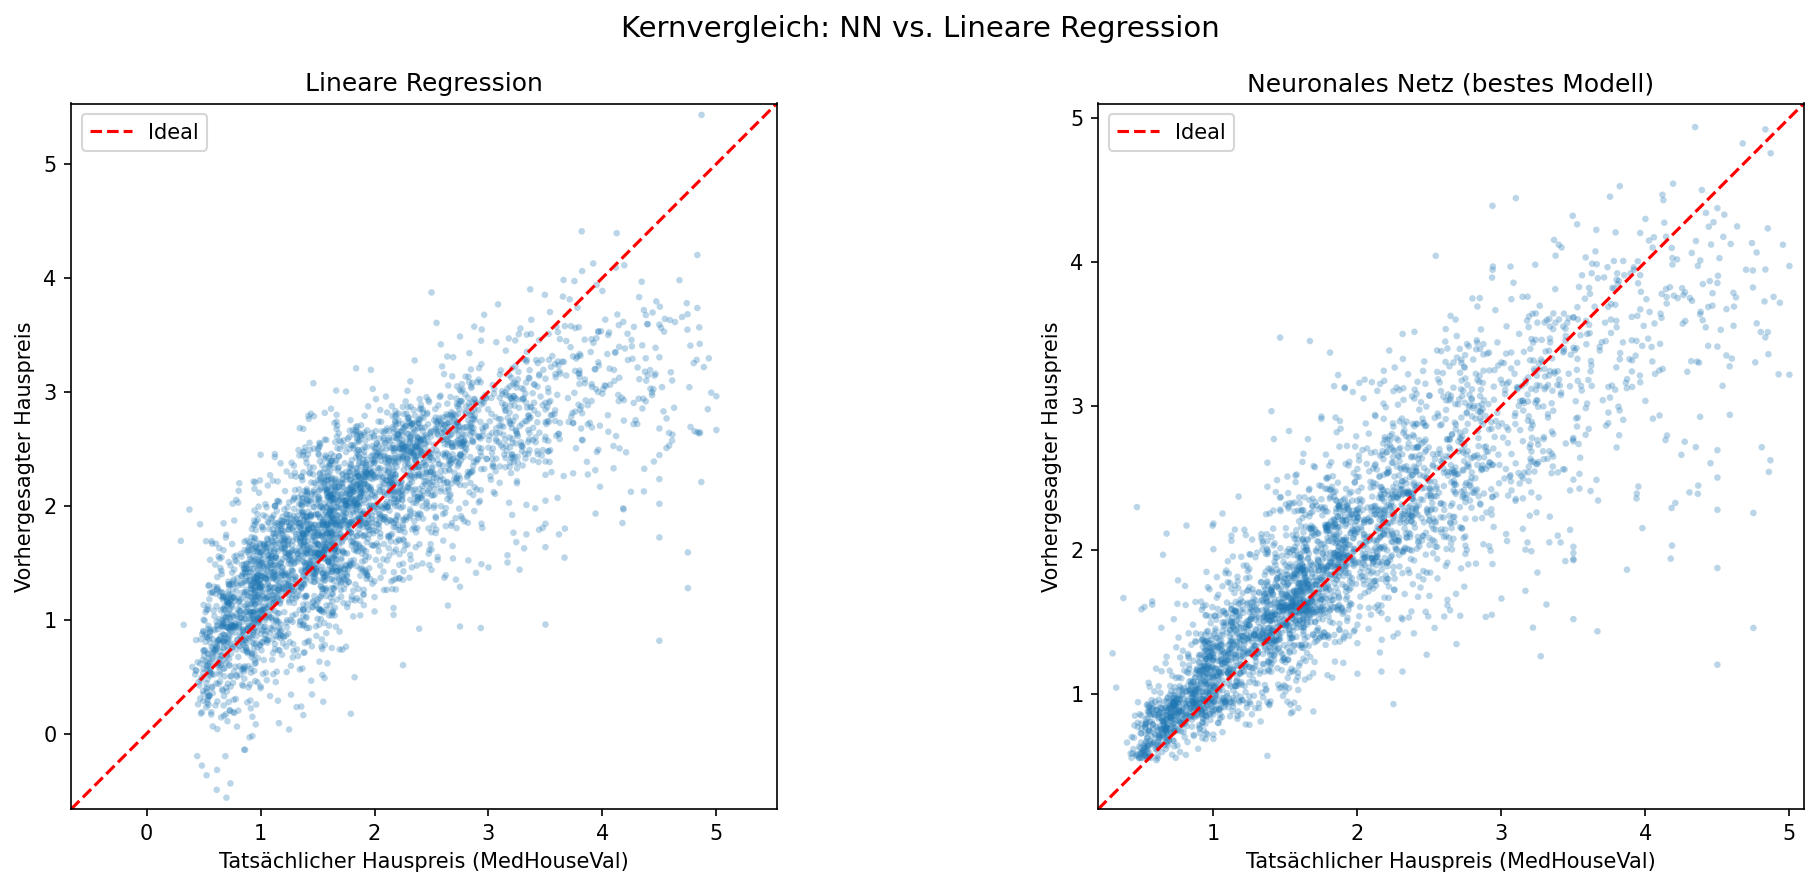
\includegraphics[width=\columnwidth]{../../results/nn_vs_linear_regression.pdf}
    \caption{Direkter Vergleich des besten neuronalen Netzes gegen die lineare Regression. Das beste Netz erreicht auf dem Testset $R^2 = 0{,}7795$ und verbessert die Baseline damit deutlich.}
    \label{fig:nn-main}
\end{figure}

\begin{table}[H]
\centering
\caption{Detaillierte Entwicklung der NN-Architekturen (Notebook Florian)}
\label{tab:nn-detail-florian}
\small
\setlength{\tabcolsep}{4pt}
\begin{tabularx}{\columnwidth}{>{\raggedright\arraybackslash}Xcc}
\toprule
\textbf{Modell} & \textbf{$R^2$ Train} & \textbf{$R^2$ Test} \\
\midrule
Lineare Regression & 0.6465 & 0.6326 \\
NN [32] & 0.7555 & 0.7427 \\
NN [64,32,16] & 0.8200 & 0.7393 \\
NN [128,64,32] & 0.8804 & 0.7171 \\
NN [128,64,32,16]+Dropout & 0.8272 & 0.7525 \\
Bestes Ergebnis (Summary) & -- & 0.7795 \\
\bottomrule
\end{tabularx}
\setlength{\tabcolsep}{6pt}
\normalsize
\end{table}

Die Tabelle zeigt den Kernpunkt meiner NN-Arbeit: Mit steigender Modellkapazit\"at steigt zun\"achst die Leistung, aber ohne Regularisierung kippt das Modell in Overfitting. Genau hier war Dropout entscheidend. Modell~3 erzielt einen sehr hohen Trainingsscore, verliert aber deutlich auf dem Testset; das tiefere Modell mit Dropout generalisiert stabiler und liefert die bessere praktische Modellg\"ute.

\begin{comment}
\begin{figure*}[t]
    \centering
    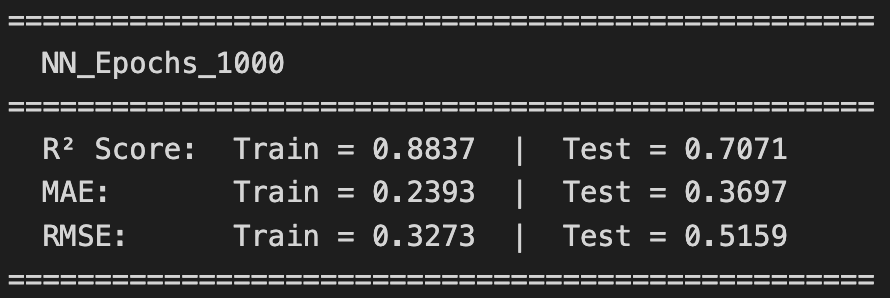
\includegraphics[width=\pairfigwidth]{../../results/overfitting 1000 Epochen.png}
    \hfill
    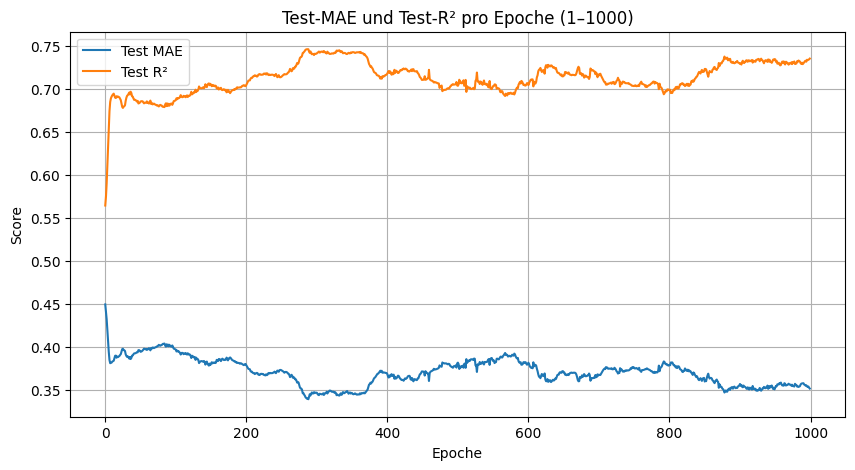
\includegraphics[width=\pairfigwidth]{../../results/MAE und R2 Test pro Epoche.png}
    \caption{Zus\"atzliche NN-Diagnostik aus den Ergebnissen: links das Overfitting-Verhalten bei sehr langen Trainingsl\"aufen, rechts die gemeinsame Entwicklung von Test-MAE und Test-$R^2$ \"uber viele Epochen. Die Kurven erkl\"aren, warum ich auf kontrollierte Regularisierung statt nur l\"angeres Training gesetzt habe.}
    \label{fig:nn-overfit-epochs}
\end{figure*}

\begin{figure*}[t]
    \centering
    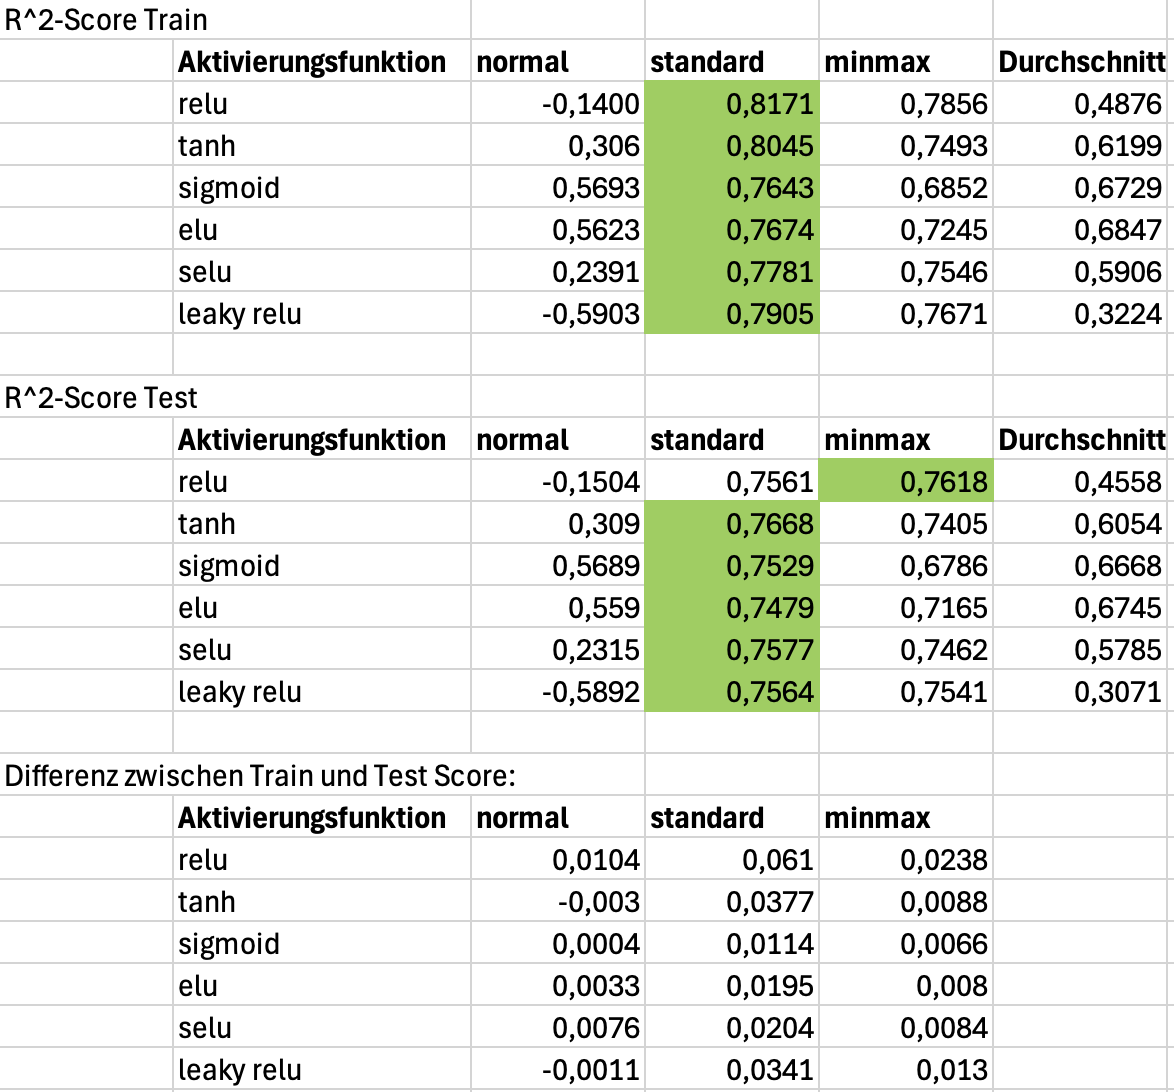
\includegraphics[width=\pairfigwidth]{../../results/Ergebnisse Untersuchung Aktivierungsfunktion.png}
    \hfill
    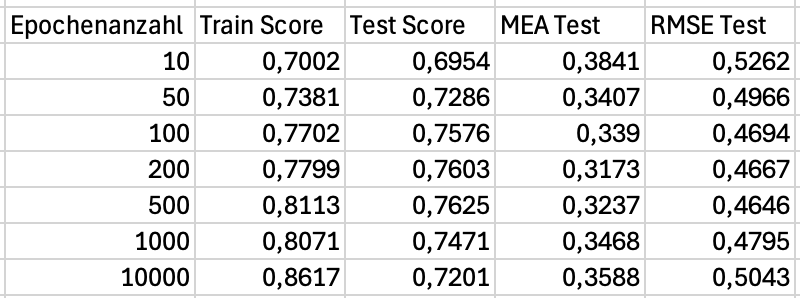
\includegraphics[width=\pairfigwidth]{../../results/epochenanzahl results.png}
    \caption{Zus\"atzliche Analyseentscheidungen: links der Einfluss verschiedener Aktivierungsfunktionen und Skalierungen, rechts die Sensitivit\"at gegen\"uber der Epochenzahl. Diese Analysen waren Teil meines systematischen Tuning-Prozesses und nicht nur isolierte Einzeltests.}
    \label{fig:nn-activation-epochs-table}
\end{figure*}
\end{comment}

Das Ergebnis ist nicht nur numerisch besser, sondern auch inhaltlich plausibel: Der California-Housing-Datensatz enth\"alt nichtlineare Abh\"angigkeiten, regionale Muster und Wechselwirkungen, die eine lineare Regression nur unvollst\"andig erfasst. Das NN kann diese Muster besser modellieren, braucht daf\"ur aber mehr Aufwand bei Architektur und Tuning \cite{russellNorvig,tfGuide,sklearnMetrics}.

\begin{figure}[H]
    \centering
    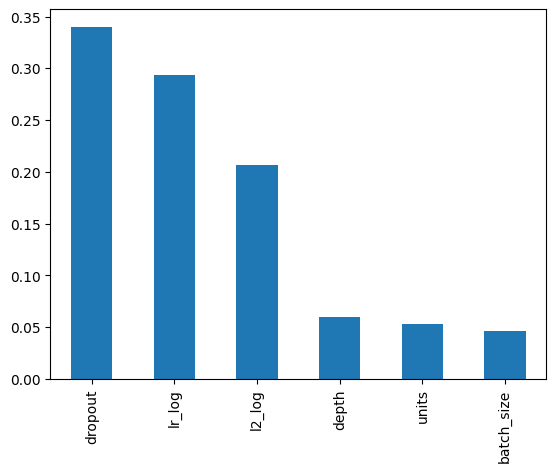
\includegraphics[width=0.7\columnwidth]{../../results/Hyperparameters_Feature_Importance.png}
    \caption{Hyperparameteranalyse des NN. Vor allem Dropout, Lernrate und L2-Regularisierung haben einen deutlichen Einfluss; reines Nachjustieren einzelner Parameter reicht daher nicht aus.}
    \label{fig:nn-hyperparams}
\end{figure}

\begin{figure}[H]
    \centering
    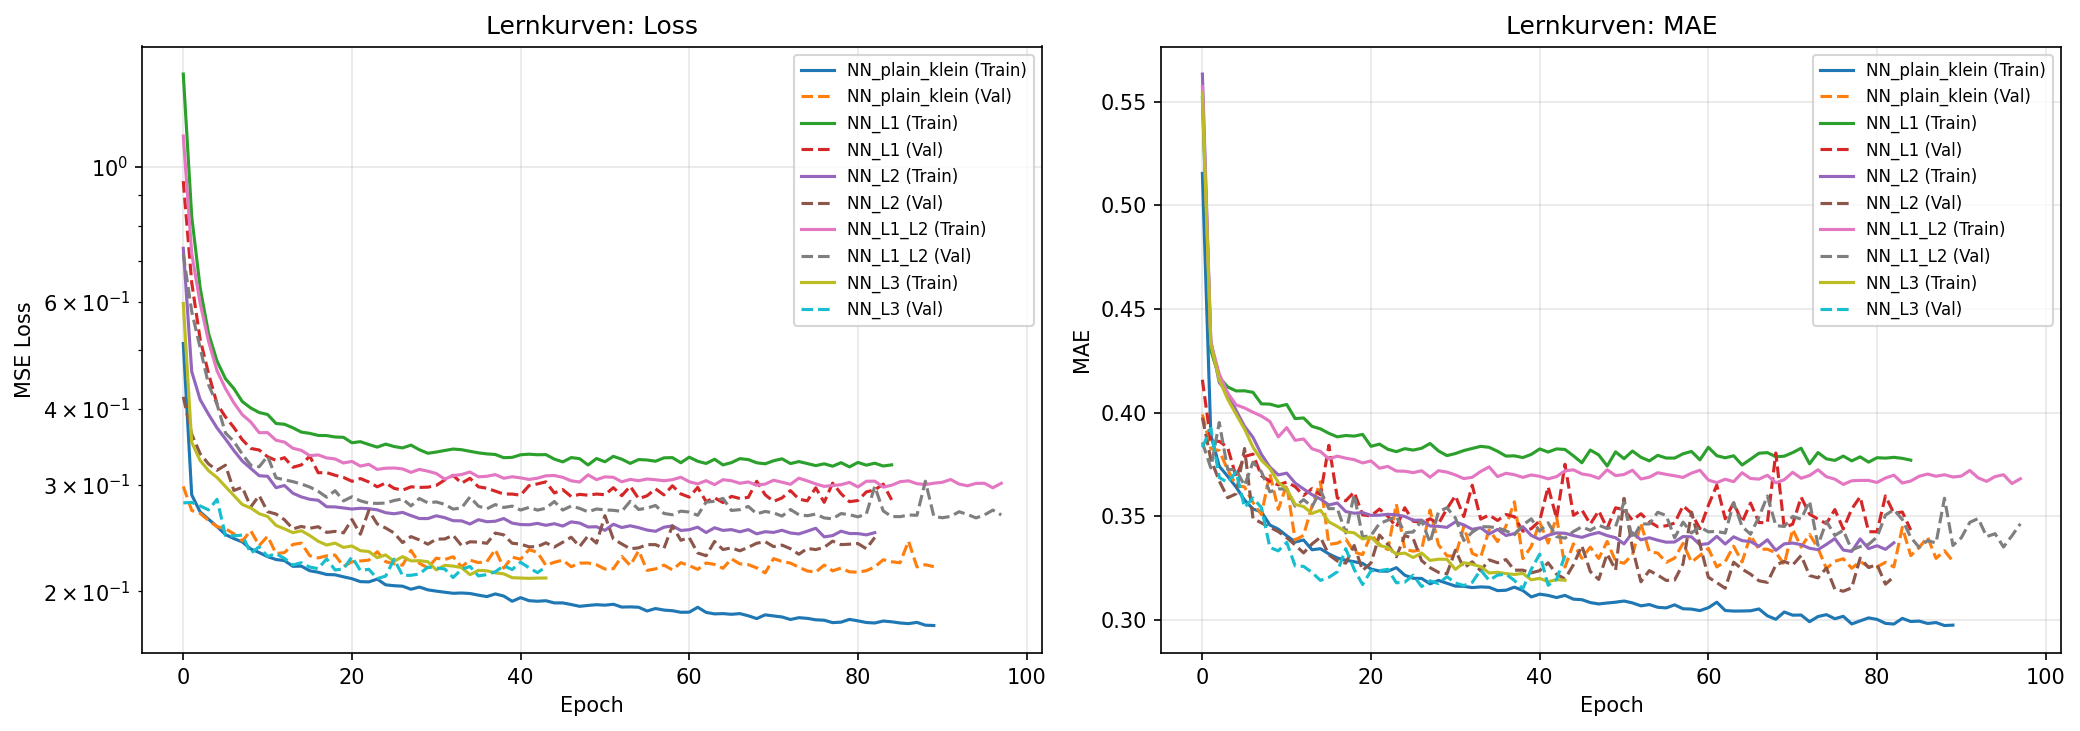
\includegraphics[width=\columnwidth]{../../results/nn_learning_curves.png}
    \caption{Lernkurven der getesteten NN-Architekturen (Train/Validation) \"uber die Epochen. Man sieht, dass gr\"o\ss{}ere Modelle den Trainingsfehler schneller reduzieren, sich die Validierung aber je nach Architektur unterschiedlich stabil entwickelt. Genau aus diesem Verlauf folgt meine zentrale Tuning-Entscheidung: Nicht nur mehr Tiefe, sondern kontrollierte Regularisierung (insbesondere Dropout) ist notwendig, um hohe Trainingsg\"ute in robuste Testleistung zu \"uberf\"uhren.}
    \label{fig:nn-learning-curves-detailed}
\end{figure}

In der Summe ist mein Eindruck klar: Das beste Modell entsteht nicht durch einen einzigen cleveren Layer, sondern durch saubere Datenbasis, stabile Evaluation, kontrollierte Regularisierung und systematisches Tuning. Genau deshalb war die frühe Infrastrukturarbeit so wichtig.

%----------------------------------------------------------
\section{Konkrete Ergebnisse und Einordnung}
%----------------------------------------------------------
Die wichtigsten quantitativen Eckpunkte meines Beitrags sind:

\begin{itemize}[leftmargin=*,itemsep=0.15em,topsep=0.15em]
    \item Lineare Regression als Baseline: $R^2_{Test} \approx 0{,}6326$.
    \item Bestes neuronales Netz: $R^2_{Test} = 0{,}7795$.
    \item Verbesserung gegen\"uber der Baseline: rund 15 Prozentpunkte beim Test-$R^2$.
    \item Zus\"atzlich sichtbar besseres Fehlerverhalten im Residuenbild und in der Vorhersage gegen den Ist-Wert.
\end{itemize}

Im Vergleich zu den klassischen Methoden war mein NN klar \"uber der linearen Baseline und auch \"uber den meisten nichtlinearen Standardmodellen aus den Grundnotebooks. Decision-Tree-Tuning liegt sichtbar unter meinem besten NN, kNN ist solide, aber ebenfalls niedriger. Ensemble-Methoden kommen nah an NN-Leistung heran; in sp\"ateren Kombinationen wurden Werte im Bereich knapp unter bzw. um 0.79 sichtbar. Damit war mein NN-Modell in der Praxis konkurrenzf\"ahig zu den starken klassischen Verfahren \cite{bergstra2012,srivastava2014}.

Auch f\"ur die Teamarbeit war mein Beitrag relevant, weil ich die Umgebung und die Arbeitsweise f\"ur alle anderen mit vorbereitet habe:

\begin{itemize}[leftmargin=*,itemsep=0.15em,topsep=0.15em]
    \item Ich habe \texttt{README.md} und \texttt{requirements.txt} so aufgebaut, dass neue Teammitglieder schneller starten konnten.
    \item Ich habe nbstripout und Git-Hooks thematisiert, damit Notebook-Outputs nicht die Versionsgeschichte verunreinigen.
    \item Ich habe Notebook-Vorlagen und Meeting-Vorlagen mit vorbereitet, damit die Gruppentreffen strukturierter dokumentiert werden konnten.
    \item Ich habe mehrfach bei Git- und VS-Code-Fragen geholfen, weil f\"ur viele im Team dies die erste Arbeit in dieser Umgebung war.
\end{itemize}

\subsection*{Bewertung der Arbeit}
Mein eigener Beitrag lag damit weniger in einem einzelnen Modell als in einer belastbaren Kette von Entscheidungen: gute Datenbasis, saubere Werkzeuge, reproduzierbare Auswertung und erst darauf aufbauend Modellierung. Genau diese Reihenfolge ist fachlich wichtig, weil sie verhindert, dass zuf\"allige Effekte als Fortschritt missverstanden werden.

%----------------------------------------------------------
\section{Einsch\"atzung der Gruppenmitglieder}
%----------------------------------------------------------
Gem\"a\ss{} Aufgabenstellung benenne ich f\"ur jedes Gruppenmitglied jeweils mindestens eine St\"arke und eine Schw\"ache, mit Fokus auf Zusammenarbeit, Arbeitsweise und Kommunikation.

\subsection*{Kolja Scriba}
\textbf{St\"arke:} Kolja war besonders am Anfang des Projekts sehr aktiv und hat fr\"uh produktive Beitr\"age geliefert. Die Abstimmung mit ihm lief sehr schnell und unkompliziert, vor allem \"uber WhatsApp, was die gemeinsame Planung deutlich erleichtert hat.

\textbf{Schw\"ache:} Durch den Umzug war seine verf\"ugbare Zeit sp\"ater eingeschr\"ankter, was die Kontinuit\"at einzelner Aufgabenphasen erschwert hat. Zus\"atzlich gab es zeitweise technische Reibung durch das Macbook-Setup.

\subsection*{Bj\"orn Becker}
\textbf{St\"arke:} Bj\"orn hat in der Endphase mit hoher Intensit\"at gearbeitet und insbesondere bei Hyperparameter-Suchen, Iterationen und Ergebnisaufbereitung viel eingebracht. Seine sp\"ate Phase war inhaltlich stark und gut dokumentiert.

\textbf{Schw\"ache:} Wegen Klausuren war sein aktiver Einstieg sp\"ater als bei den anderen. Dadurch mussten einige Grundlagen zuerst nachgezogen werden, bevor er voll in die Modellarbeit einsteigen konnte.

\subsection*{Felix Hollfoth}
\textbf{St\"arke:} Felix H. hatte sehr viel fachliche Sicherheit bei neuronalen Netzen und konnte viele inhaltliche Impulse geben, etwa bei Random Search, Feature-Selektion und Lernratenstrategien.

\textbf{Schw\"ache:} Durch den hohen inhaltlichen Anspruch waren seine Arbeiten teils schwerer f\"ur alle Teammitglieder sofort anschlussf\"ahig. F\"ur die Gruppe bedeutete das zus\"atzlichen Abstimmungsbedarf in der \"Ubergabe.

\subsection*{Felix Neumann (Sprecher)}
\textbf{St\"arke:} Felix N. hat als Sprecher die Organisation in der Schlussphase sehr zuverl\"assig getragen und die Abgabewege, Terminfragen und Konsolidierung sauber koordiniert.

\textbf{Schw\"ache:} Auch bei ihm gab es durch das Macbook-Setup zeitweise technische H\"urden im Umfeld TensorFlow/Python-Versionen, was punktuell Zusatzaufwand in der Abstimmung erzeugte.

\subsection*{Selbsteinsch\"atzung (Florian Adamczyk)}
\textbf{St\"arke:} Ich habe die Vorarbeit fr\"uh und umfassend \"ubernommen und damit den technischen Unterbau geliefert, auf dem die gesamte Modellarbeit aufbauen konnte. Dazu kamen schneller Support bei Git/VS Code sowie hohe Erreichbarkeit f\"ur Abstimmungen.

\textbf{Schw\"ache:} Weil ich viel Infrastruktur- und Supportarbeit gemacht habe, blieb weniger Zeit f\"ur tiefes eigenes Hyperparameter-Tuning in der allerletzten Phase als in einem reinen Einzelprojekt m\"oglich gewesen w\"are.

%----------------------------------------------------------
\section{Fazit}
%----------------------------------------------------------
Ich sehe meinen Beitrag als die technische und methodische Grundlage des Projekts. Die sp\"atere Modellarbeit der Gruppe konnte nur deshalb sinnvoll verglichen werden, weil ich die Vorarbeit auf einheitliche Daten, Metriken, Plots und Projektstruktur ausgerichtet habe. Gleichzeitig habe ich mit dem eigenen NN-Notebook gezeigt, dass sich der California-Housing-Datensatz mit einem gut regularisierten Netz deutlich besser modellieren l\"asst als mit einer linearen Regression.

Die wichtigste Schlussfolgerung ist deshalb zweistufig: Erstens ist die Vorarbeit kein Nebenprodukt, sondern Voraussetzung f\"ur belastbare Ergebnisse. Zweitens ist das neuronale Netz im Projekt nicht nur "das letzte Modell", sondern der methodische Abschluss einer sauberen Modellkette, die bei EDA und Baseline beginnt.

%----------------------------------------------------------
\section*{Quellen und Hilfsmittel}
Die externen Quellen werden im Flie\ss{}text mit \texttt{\textbackslash cite\{...\}} referenziert und nachfolgend vollst\"andig dokumentiert. Als Entwicklungs- und Analysewerkzeuge wurden insbesondere Python, TensorFlow/Keras, scikit-learn, pandas, numpy, matplotlib, seaborn, Jupyter und VS Code eingesetzt. Der Umgang mit Notebook-Outputs im Git-Workflow wurde mit \texttt{nbstripout} organisiert \cite{nbstripout}.

Der Einsatz generativer KI erfolgte unterst\"utzend f\"ur Strukturfeedback, sprachliche Straffung und Formulierungsalternativen; die inhaltlichen Aussagen, Metriken, Tabellenwerte und Abbildungsinterpretationen stammen aus den eigenen Notebooks und Resultatdateien.
\printbibliography[heading=none]

\newpage

%----------------------------------------------------------
% Anhang: Logbuch
%----------------------------------------------------------
\section*{Anhang: Logbuch}
Das vollst\"andige Logbuch ist als Pflichtanhang beigef\"ugt und dokumentiert die Arbeitsschritte chronologisch.

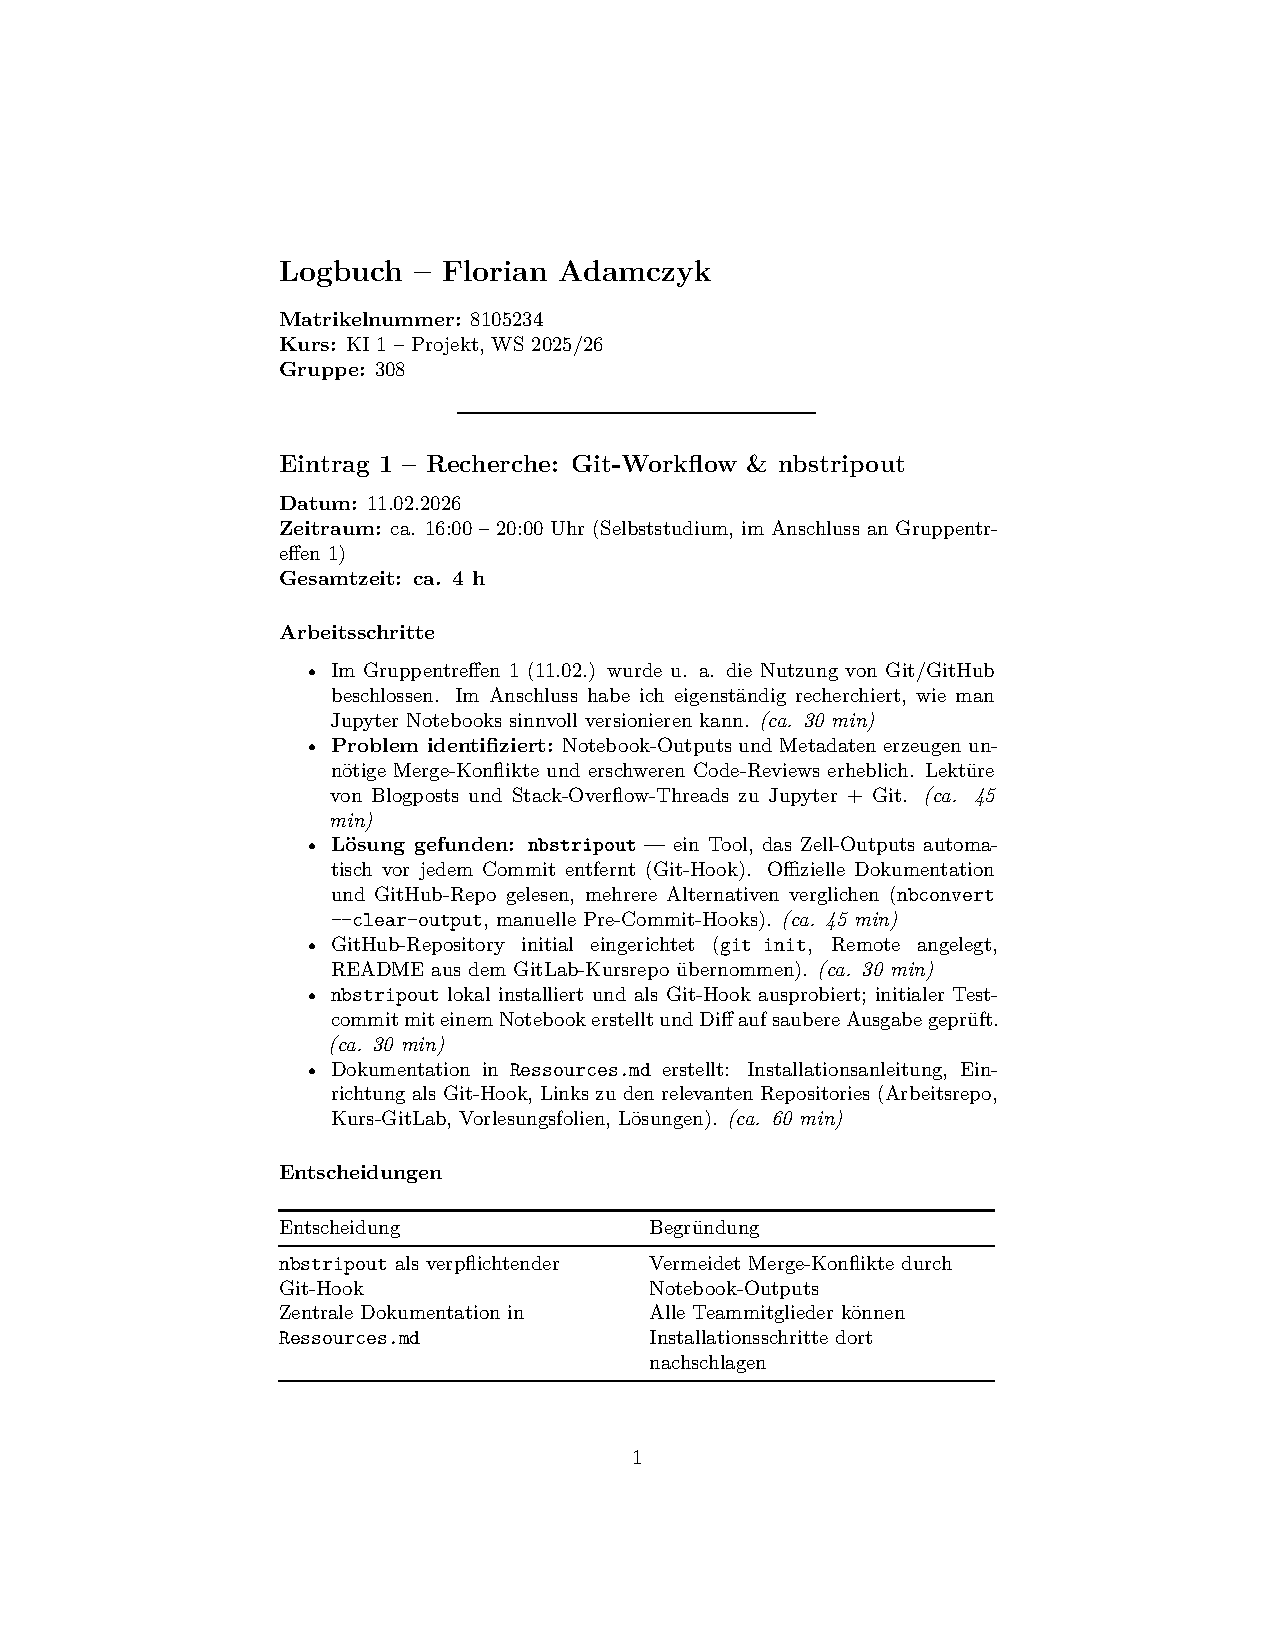
\includepdf[pages=-,pagecommand={\thispagestyle{plain}}]{../Logbuch_Florian_Adamczyk.pdf}

\end{document}